\documentclass{ximera}
\usepackage{epsfig}

\graphicspath{
  {./}
  {figures/}
}


\usepackage{morewrites}

%\newcounter{ccounter}
%\setcounter{ccounter}{1}
%\newcommand{\Chapter}[1]{\setcounter{chapter}{\arabic{ccounter}}\chapter{#1}\addtocounter{ccounter}{1}}

%\newcommand{\section}[1]{\section{#1}\setcounter{thm}{0}\setcounter{equation}{0}}

%\renewcommand{\theequation}{\arabic{chapter}.\arabic{section}.\arabic{equation}}
%\renewcommand{\thefigure}{\arabic{chapter}.\arabic{figure}}
%\renewcommand{\thetable}{\arabic{chapter}.\arabic{table}}

%\newcommand{\Sec}[2]{\section{#1}\markright{\arabic{ccounter}.\arabic{section}.#2}\setcounter{equation}{0}\setcounter{thm}{0}\setcounter{figure}{0}}

\newcommand{\Sec}[2]{\section{#1}}

\setcounter{secnumdepth}{2}
%\setcounter{secnumdepth}{1} 

%\newcounter{THM}
%\renewcommand{\theTHM}{\arabic{chapter}.\arabic{section}}

\newcommand{\trademark}{{R\!\!\!\!\!\bigcirc}}
%\newtheorem{exercise}{}

\newcommand{\dfield}{{\sf dfield9}}
\newcommand{\pplane}{{\sf pplane9}}

\newcommand{\EXER}{\section*{Exercises}}%\vspace*{0.2in}\hrule\small\setcounter{exercise}{0}}
\newcommand{\CEXER}{}%\vspace{0.08in}\begin{center}Computer Exercises\end{center}}
\newcommand{\TEXER}{} %\vspace{0.08in}\begin{center}Hand Exercises\end{center}}
\newcommand{\AEXER}{} %\vspace{0.08in}\begin{center}Hand Exercises\end{center}}

% BADBAD: \newcommand{\Bbb}{\bf}

\newcommand{\R}{\mbox{$\Bbb{R}$}}
\newcommand{\C}{\mbox{$\Bbb{C}$}}
\newcommand{\Z}{\mbox{$\Bbb{Z}$}}
\newcommand{\N}{\mbox{$\Bbb{N}$}}
\newcommand{\D}{\mbox{{\bf D}}}
\usepackage{amssymb}
%\newcommand{\qed}{\hfill\mbox{\raggedright$\square$} \vspace{1ex}}
%\newcommand{\proof}{\noindent {\bf Proof:} \hspace{0.1in}}

\newcommand{\setmin}{\;\mbox{--}\;}
\newcommand{\Matlab}{{M\small{AT\-LAB}} }
\newcommand{\Matlabp}{{M\small{AT\-LAB}}}
\newcommand{\computer}{\Matlab Instructions}
\newcommand{\half}{\mbox{$\frac{1}{2}$}}
\newcommand{\compose}{\raisebox{.15ex}{\mbox{{\scriptsize$\circ$}}}}
\newcommand{\AND}{\quad\mbox{and}\quad}
\newcommand{\vect}[2]{\left(\begin{array}{c} #1_1 \\ \vdots \\
 #1_{#2}\end{array}\right)}
\newcommand{\mattwo}[4]{\left(\begin{array}{rr} #1 & #2\\ #3
&#4\end{array}\right)}
\newcommand{\mattwoc}[4]{\left(\begin{array}{cc} #1 & #2\\ #3
&#4\end{array}\right)}
\newcommand{\vectwo}[2]{\left(\begin{array}{r} #1 \\ #2\end{array}\right)}
\newcommand{\vectwoc}[2]{\left(\begin{array}{c} #1 \\ #2\end{array}\right)}



\newcommand{\inv}{^{-1}}
\newcommand{\CC}{{\cal C}}
\newcommand{\CCone}{\CC^1}
\newcommand{\Span}{{\rm span}}
\newcommand{\rank}{{\rm rank}}
\newcommand{\trace}{{\rm tr}}
\newcommand{\RE}{{\rm Re}}
\newcommand{\IM}{{\rm Im}}
\newcommand{\nulls}{{\rm null\;space}}

\newcommand{\dps}{\displaystyle}
\newcommand{\arraystart}{\renewcommand{\arraystretch}{1.8}}
\newcommand{\arrayfinish}{\renewcommand{\arraystretch}{1.2}}
\newcommand{\Start}[1]{\vspace{0.08in}\noindent {\bf Section~\ref{#1}}}
\newcommand{\exer}[1]{\noindent {\bf \ref{#1}}}
\newcommand{\ans}{}
\newcommand{\matthree}[9]{\left(\begin{array}{rrr} #1 & #2 & #3 \\ #4 & #5 & #6
\\ #7 & #8 & #9\end{array}\right)}
\newcommand{\cvectwo}[2]{\left(\begin{array}{c} #1 \\ #2\end{array}\right)}
\newcommand{\cmatthree}[9]{\left(\begin{array}{ccc} #1 & #2 & #3 \\ #4 & #5 &
#6 \\ #7 & #8 & #9\end{array}\right)}
\newcommand{\vecthree}[3]{\left(\begin{array}{r} #1 \\ #2 \\
#3\end{array}\right)}
\newcommand{\cvecthree}[3]{\left(\begin{array}{c} #1 \\ #2 \\
#3\end{array}\right)}
\newcommand{\cmattwo}[4]{\left(\begin{array}{cc} #1 & #2\\ #3
&#4\end{array}\right)}

\newcommand{\Matrix}[1]{\ensuremath{\left(\begin{array}{rrrrrrrrrrrrrrrrrr} #1 \end{array}\right)}}

\newcommand{\Matrixc}[1]{\ensuremath{\left(\begin{array}{cccccccccccc} #1 \end{array}\right)}}



\renewcommand{\labelenumi}{\theenumi)}
\newenvironment{enumeratea}%
{\begingroup
 \renewcommand{\theenumi}{\alph{enumi}}
 \renewcommand{\labelenumi}{(\theenumi)}
 \begin{enumerate}}
 {\end{enumerate}\endgroup}



\newcounter{help}
\renewcommand{\thehelp}{\thesection.\arabic{equation}}

%\newenvironment{equation*}%
%{\renewcommand\endequation{\eqno (\theequation)* $$}%
%   \begin{equation}}%
%   {\end{equation}\renewcommand\endequation{\eqno \@eqnnum
%$$\global\@ignoretrue}}

%\input{psfig.tex}

\author{Martin Golubitsky and Michael Dellnitz}

%\newenvironment{matlabEquation}%
%{\renewcommand\endequation{\eqno (\theequation*) $$}%
%   \begin{equation}}%
%   {\end{equation}\renewcommand\endequation{\eqno \@eqnnum
% $$\global\@ignoretrue}}

\newcommand{\soln}{\textbf{Solution:} }
\newcommand{\exercap}[1]{\centerline{Figure~\ref{#1}}}
\newcommand{\exercaptwo}[1]{\centerline{Figure~\ref{#1}a\hspace{2.1in}
Figure~\ref{#1}b}}
\newcommand{\exercapthree}[1]{\centerline{Figure~\ref{#1}a\hspace{1.2in}
Figure~\ref{#1}b\hspace{1.2in}Figure~\ref{#1}c}}
\newcommand{\para}{\hspace{0.4in}}

\renewenvironment{solution}{\suppress}{\endsuppress}

\ifxake
\newenvironment{matlabEquation}{\begin{equation}}{\end{equation}}
\else
\newenvironment{matlabEquation}%
{\let\oldtheequation\theequation\renewcommand{\theequation}{\oldtheequation*}\begin{equation}}%
  {\end{equation}\let\theequation\oldtheequation}
\fi

\makeatother

\begin{document}

\noindent In Exercises~\ref{c9.6.3a} -- \ref{c9.6.3b}, consider the system 
of differential equations \eqref{E:infinity}.
\begin{matlabEquation}  \label{E:infinity}
\begin{array}{rcl}
\dot{x} & = & y \\
\dot{y} & = & -x +\rho y + \frac{1}{2}\cos(x)y
\end{array}
\end{matlabEquation}
\begin{exercise} \label{c9.6.3a}
How many periodic solutions does \eqref{E:infinity} appear to have 
when $\rho=0$?  Be careful when answering this question.  First use 
{\pplane} to determine the number of limit cycles on the square 
$-\ell \leq x,y \leq\ell$ when $\ell=2$.  Then compute with $\ell=10$ and 
$\ell=40$.

\begin{solution}

\ans The system appears to have an infinite number of limit cycles
as the size of the computation area increases.

\soln In the region $-2 \leq x,y \leq 2$, the system appears to have no
limit cycles.  However, in the region $-10 \leq x,y \leq 10$, there are
four limit cycles, and there are more in the larger region $-40 \leq x,y
\leq 40$.  Figure~\ref{c9.6.3a} shows the system with $\rho = 0$ on the
square $-10 \leq x,y \leq 10$.

\end{solution}
\end{exercise}
\begin{exercise} \label{c9.6.3b}
Find the number of limit cycles to \eqref{E:infinity} on the square 
with $\ell=7$ when $\rho=0.06$ and when $\rho=0.07$.  Has a bifurcation
 occurred between these two values of $\rho$ and, if so, what kind of 
bifurcation?

\begin{solution}

Figure~\ref{c9.6.3b}a shows the system with $\rho = 0.06$, and 
Figure~\ref{c9.6.3b}b shows the system with $\rho = 0.07$.  The system
has two periodic solutions at $\rho = 0.06$, and none at $\rho = 0.07$.
A saddle node bifurcation for periodic solutions occurs between these
two values of $\rho$.

\begin{figure}[htb]
                       \centerline{%
                       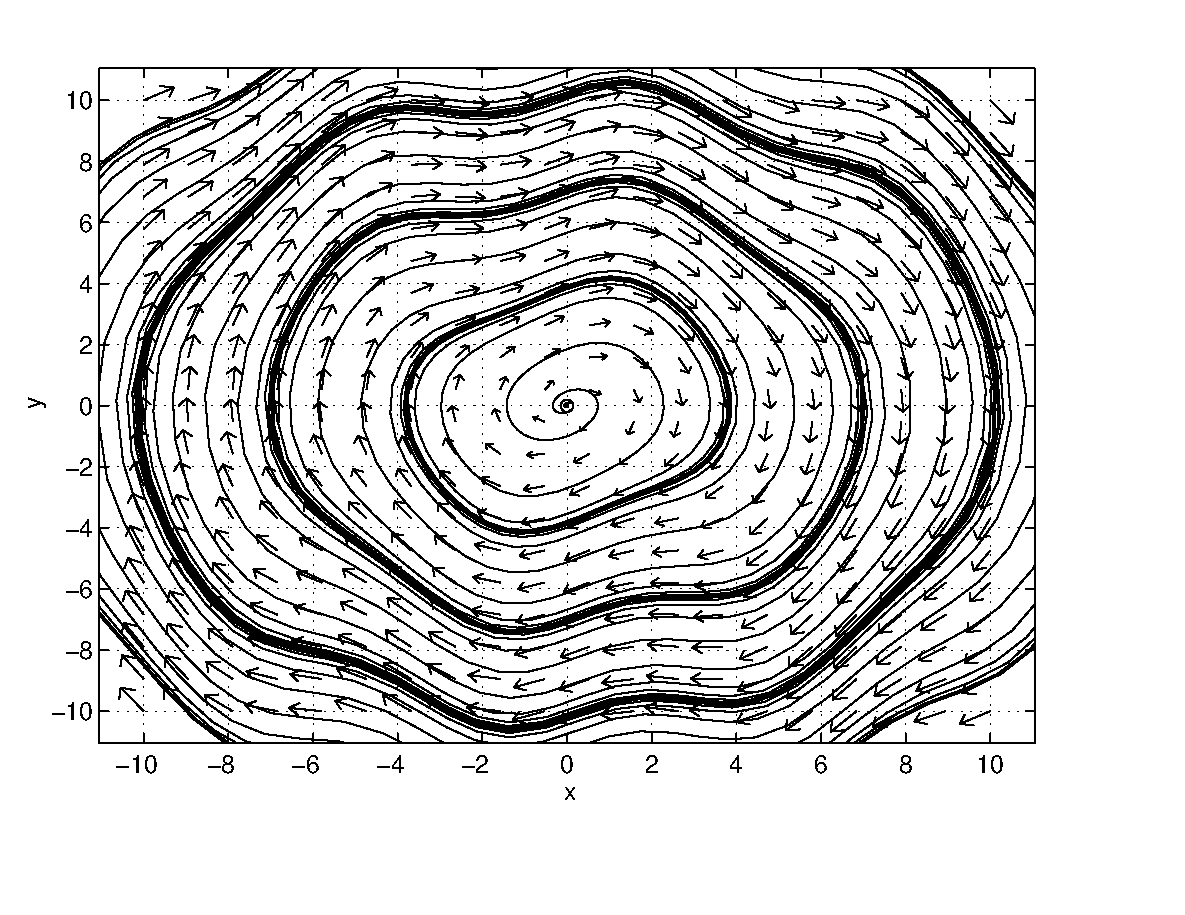
\psfig{file=exfigure/9-6-3a.eps,width=1.8in}
                       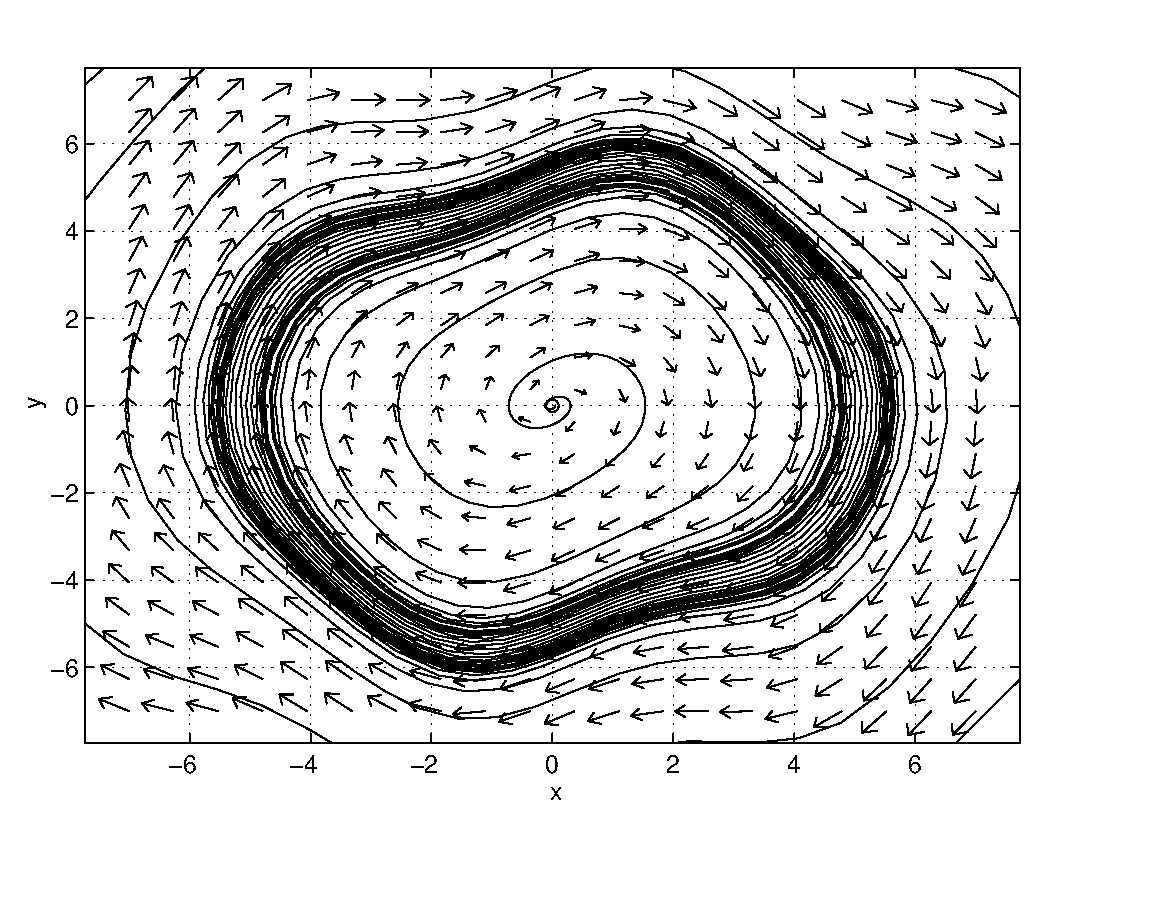
\psfig{file=exfigure/9-6-3b.eps,width=1.8in}
                       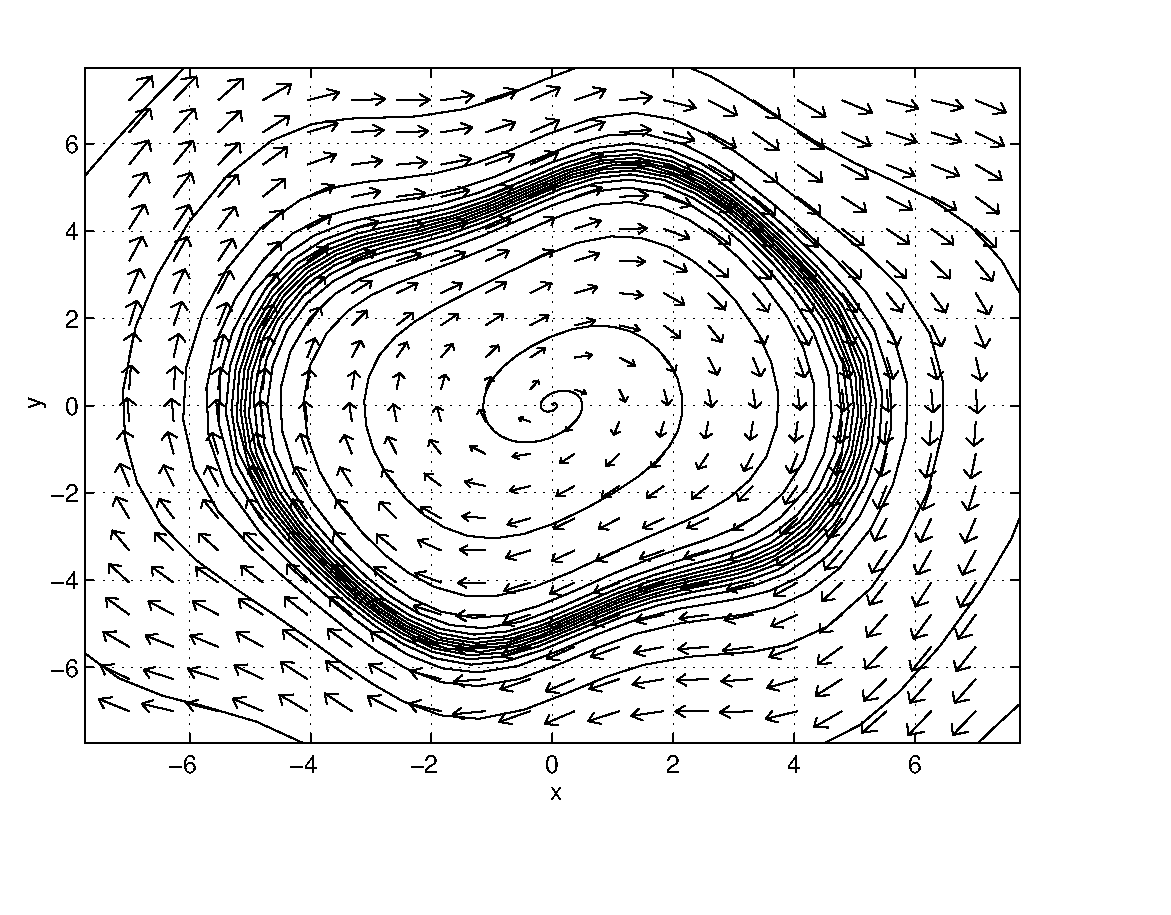
\psfig{file=exfigure/9-6-3c.eps,width=1.8in}}
		\centerline{$\rho = 0$\hspace{1.3in}$\rho = 0.06$
\hspace{1.3in}$\rho = 0.07$}
		\centerline{Figure~\ref{c9.6.3a}\hspace{1.2in}
Figure~\ref{c9.6.3b}a\hspace{1.2in}Figure~\ref{c9.6.3b}b}
\end{figure}

\end{solution}
\end{exercise}
\end{document}
